% F1: AXIOM encoder + per-slice Q-heads (left) and the federated
% training loop (right). Standalone-compilable for iteration; \input{}
% into the paper body. Mirrors Papers_4-5/Paper_4/figures/fig1_architecture.tex's
% style conventions (box/arrow styles, font, palette).
\documentclass[tikz,border=2pt]{standalone}
\usepackage{amsmath}
\usetikzlibrary{arrows.meta,positioning,fit,backgrounds}

\begin{document}
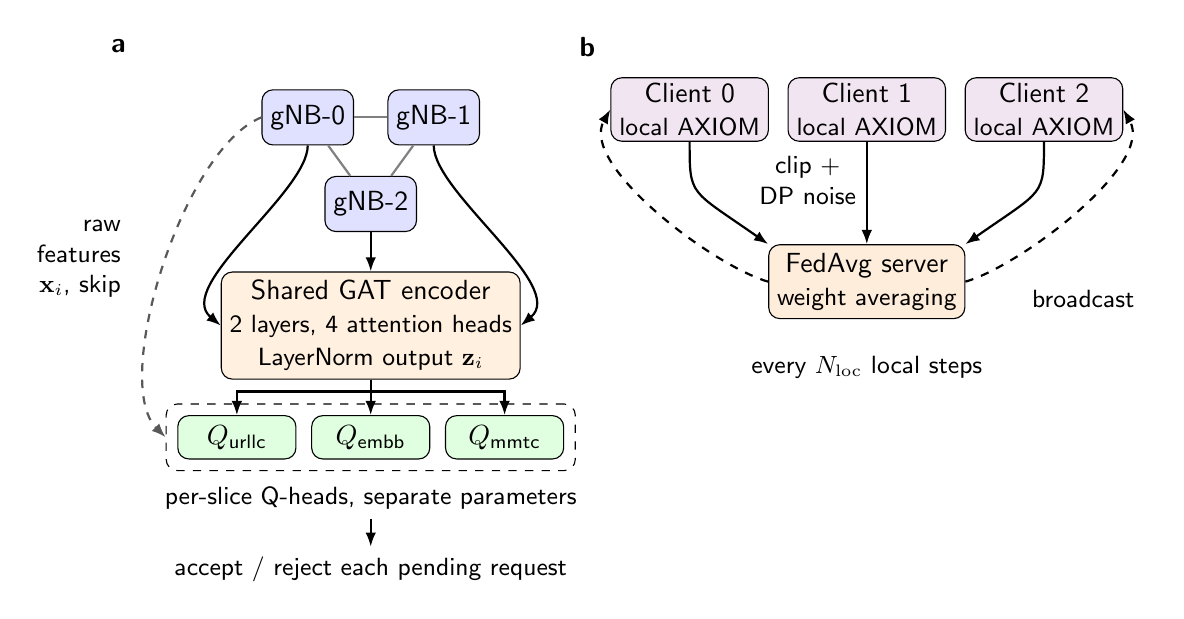
\begin{tikzpicture}[
  font=\sffamily\normalsize,
  box/.style={draw, rounded corners, minimum height=0.7cm, align=center, inner sep=3pt},
  node1/.style={box, fill=blue!12, minimum width=1.0cm},
  node2/.style={box, fill=blue!12, minimum width=1.0cm},
  node3/.style={box, fill=blue!12, minimum width=1.0cm},
  encoder/.style={box, fill=orange!12, minimum width=2.6cm},
  qhead/.style={box, fill=green!12, minimum width=1.5cm, minimum height=0.55cm},
  client/.style={box, fill=violet!10, minimum width=1.8cm, inner sep=2pt},
  server/.style={box, fill=orange!14, minimum width=2.0cm},
  arrow/.style={-{Latex[length=1.8mm]}, thick},
  dashedarrow/.style={-{Latex[length=1.8mm]}, thick, dashed},
]

% ===== Left half: AXIOM per-agent pipeline =====
\node[font=\sffamily\bfseries] (lefttitle) at (-3.2,3.0) {a};

% 3-gNB fully-connected graph
\node[node1] (n1) at (-0.8,2.1) {gNB-0};
\node[node2] (n2) at (0.8,2.1) {gNB-1};
\node[node3] (n3) at (0,1.0) {gNB-2};
\draw[thick, gray] (n1) -- (n2);
\draw[thick, gray] (n1) -- (n3);
\draw[thick, gray] (n2) -- (n3);

\node[encoder, below=0.5cm of n3] (gat) {Shared GAT encoder\\\small 2 layers, 4 attention heads\\\small LayerNorm output $\mathbf{z}_i$};
\draw[arrow] (n1.south) .. controls +(0,-0.6) and +(-0.6,0.5) .. (gat.west);
\draw[arrow] (n2.south) .. controls +(0,-0.6) and +(0.6,0.5) .. (gat.east);
\draw[arrow] (n3.south) -- (gat.north);

\node[qhead, below=0.45cm of gat, xshift=-1.7cm] (q1) {$Q_{\text{urllc}}$};
\node[qhead, below=0.45cm of gat] (q2) {$Q_{\text{embb}}$};
\node[qhead, below=0.45cm of gat, xshift=1.7cm] (q3) {$Q_{\text{mmtc}}$};
\draw[arrow] (gat.south) -- ++(0,-0.15) -| (q1.north);
\draw[arrow] (gat.south) -- (q2.north);
\draw[arrow] (gat.south) -- ++(0,-0.15) -| (q3.north);
\node[draw, dashed, rounded corners, fit=(q1)(q2)(q3), inner sep=4pt] (qbox) {};
\node[below=0.08cm of qbox, font=\sffamily\small] (qlab) {per-slice Q-heads, separate parameters};

\node[below=0.35cm of qlab, font=\sffamily\small, align=center] (action) {accept / reject each pending request};
% raw-feature skip into the heads: Q_k([z_i, x_i])
\draw[dashedarrow, gray!70!black] (n1.west) .. controls +(-1.0,-0.4) and +(-0.7,0.7) .. (qbox.west);
\node[anchor=east, font=\sffamily\small, align=right] at (-3.05,0.3) {raw\\features\\$\mathbf{x}_i$, skip};
\draw[arrow] (qlab.south) -- (action.north);

% ===== Right half: federated training loop =====
\node[font=\sffamily\bfseries] (righttitle) at (2.75,3.0) {b};

\node[client, minimum width=2.0cm] (c1) at (4.05,2.2) {Client 0\\\small local AXIOM};
\node[client, minimum width=2.0cm] (c2) at (6.3,2.2) {Client 1\\\small local AXIOM};
\node[client, minimum width=2.0cm] (c3) at (8.55,2.2) {Client 2\\\small local AXIOM};

\node[server, below=1.3cm of c2] (server) {FedAvg server\\\small weight averaging};

\draw[arrow] (c1.south) .. controls +(0,-0.7) and +(-1.0,0.7) .. (server.north west);
\draw[arrow] (c2.south) -- (server.north);
\draw[arrow] (c3.south) .. controls +(0,-0.7) and +(1.0,0.7) .. (server.north east);

\draw[dashedarrow] (server.west) .. controls +(-0.7,0.2) and +(-0.4,-0.7) .. (c1.west);
\draw[dashedarrow] (server.east) .. controls +(0.7,0.2) and +(0.4,-0.7) .. (c3.east);
\node[font=\sffamily\small, align=center] at (5.55,1.3) {clip +\\DP noise};
\node[font=\sffamily\small] at (9.05,-0.2) {broadcast};

\node[below=0.35cm of server, font=\sffamily\small, align=center] {every $N_{\mathrm{loc}}$ local steps};

\end{tikzpicture}
\end{document}
